\documentclass{article}
%http://ctan.unixbrain.com/macros/latex/contrib/bytefield/
%\usepackage[margin=0.5in]{geometry}
%\usepackage{titling}
%\usepackage[compact]{titlesec}
\usepackage{fancyhdr} % custom headers
\usepackage{lastpage} % determine the last page for the footer
\usepackage{extramarks} % header footer
\usepackage{bytefield}
\usepackage{graphicx}
\usepackage{float}
\usepackage{url}
\usepackage[pdfborder={0 0 0}]{hyperref}
\usepackage[table]{xcolor}
\usepackage{microtype}
\usepackage[font={scriptsize,bf}]{caption}
\usepackage{booktabs}
\usepackage{listings}
\usepackage[table]{xcolor}

% margins
\topmargin=-0.45in
\evensidemargin=0in
\oddsidemargin=0in
\textwidth=6.5in
\textheight=9.0in
\headsep=0.25in

% line spacing
%\linespread{1.1}


% reduce spacing after figures
%\setlength{\belowcaptionskip}{-\baselineskip}

% setup header and footer
\pagestyle{fancy}
\lfoot{Sega Game Gear on a Chip}
\cfoot{}
\rfoot{Page\ \thepage\ of \protect\pageref{LastPage}}
\fancyhead[LE,RO]{\slshape \rightmark}
\fancyhead[LO,RE]{\slshape \leftmark}
\renewcommand\headrulewidth{0.4pt} % size of the header rule
\renewcommand\footrulewidth{0.4pt} % size of the footer rule

% remove indentation from paragraphs
\setlength\parindent{0pt}

% syntax highlighting
\definecolor{sh_comment}{rgb}{0.12, 0.38, 0.18}
\definecolor{sh_keyword}{rgb}{0.37, 0.08, 0.25}
\definecolor{sh_string}{rgb}{0.06, 0.10, 0.98}

\lstset{
    language=C,
    numbers=left,
    numberstyle=\tiny,
    frame=tb,
    showstringspaces=false,
    captionpos=b,
    stringstyle=\color{sh_string},
    keywordstyle = \color{sh_keyword}\bfseries,
    commentstyle=\color{sh_comment}\itshape,
    basicstyle=\small\sffamily,
    numbersep=-5pt,
    belowskip=-\parskip,
    aboveskip=\baselineskip
}

\newcolumntype{L}[1]{>{\raggedright\let\newline\\\arraybackslash\hspace{0pt}}m{#1}}
\newcolumntype{C}[1]{>{\centering\let\newline\\\arraybackslash\hspace{0pt}}m{#1}}
\newcolumntype{R}[1]{>{\raggedleft\let\newline\\\arraybackslash\hspace{0pt}}m{#1}}

\definecolor{lightgray}{gray}{0.9}
\definecolor{darkgreen}{RGB}{0, 150, 0}
\definecolor{darkred}{RGB}{150, 0, 0}
\definecolor{darkyellow}{RGB}{140, 140, 0}

\title{
    \vspace{2in}
    \textbf{Sega Game Gear on a Chip}\\
    Design Report
    \vspace{3in}
}
\author{ Max Thrun | Samir Silbak}
\date{Fall 2012}

\begin{document}
\maketitle

\newpage
\parskip = 0.4\baselineskip
\tableofcontents

% empty line between paragraphs
\parskip = 0.5\baselineskip

\newpage

\section{Executive Summary}

The goal of this project is to provide a case study on re-implementing a legacy
computer system in a Field Programmable Gate Array (FPGA). Our project centers
around re-implement the Sega Game Gear (GG) which is a hand held game console
released in 1991. Each digital component in the original Sega Game Gear was
identified and understood based on official and 3rd party descriptions and
specifications of their operation. Using these references we reimplemented a
majority of the original Sega Game Gear hardware in a hardware description
language (Verilog) and were successfully able to run original game ROMs on an
Altera DE1 FPGA development board.

\section{Background}

As computer systems age it is often impossible to keep physically maintaining
them.  For many legacy systems you cannot buy replacement parts and finding
people who have the skills to repair the original hardware is difficult. By
re-implementing these systems in a Field Programmable Gate Array (FPGA) you can
replace old multi-chip solutions with a single chip implementation that is
maintained in software. This allows you to future proof the existing design and
even extend its functionality. This project is a case study on re-implementing
an old game console, the Sega Game Gear, in a FPGA.

\section{Design Process}

Being that our project is a re-implementation and not a completely new design
in the traditional sense a majority of our design process revolved around
understanding the original system, breaking it down, and understanding the
components. In order to focus our efforts we attempted to split up and
prioritize each of the components of the system. We determined that we could
implement the CPU and it's associated memory separate from the video and audio
components. Once that was determined we prioritized the components in each
subsystem based on how important they are to the overall system and their
dependencies on each other.

\begin{table}[H]
    \parbox{.45\linewidth}{
    \begin{tabular}{cl}
        \toprule
        \textbf{Priority} & \textbf{Component} \\
        \midrule
        1 & Flash Memory Interface \\
        2 & System RAM \\
        3 & Memory Management Unit (MMU) \\
        4 & Z80 \\
        5 & Cartridge Mapper \\
          &\\
        \bottomrule
    \end{tabular}
    \caption{CPU \& Memory Implementation Priority}
}
\hfill
\parbox{.45\linewidth}{
    \begin{tabular}{cl}
        \toprule
        \textbf{Priority} & \textbf{Component} \\
        \midrule
        1 & VGA Controller \\
        2 & Background Tiles + VRAM \\
        3 & Video Display Processor Logic \\
        4 & Sprites \\
        5 & Controller Input \\
        6 & Sound \\
        \bottomrule
    \end{tabular}
    \caption{Video \& Sound Implementation Priority}
}
\end{table}

For the CPU subsystem the first step is to get a program (also called ROM
throughout this document) onto the flash memory chip on our development board.
Once we have a program loaded in we could then add the system RAM and the
memory management unit that selects between the too. After that we were ready
to implement the main CPU, the Zilog Z80. We determined the implementation of
the Zilog Z80 to be outside the scope of our project and utilized an open
source implementation called the TV80.  At this point we were able to run
custom programs and verify the functionality of the CPU subsystem.

For the Video and Sound subsystem the first thing that needed to be implemented
was a VGA controller to drive a VGA computer monitor. Once that was complete
the next step was to implement VRAM and the background tile render. Since the
development of this subsystem was independent of the CPU subsystem we obtained
VRAM dumps from an emulator on the computer (discussed in detail in later
sections) and used this dump to initialize the VRAM on the FPGA. This allowed
us to work off of a known, static, VRAM instead of relying on the CPU subsystem
to be correct. Basically, this technique allowed us to independently prove out
the video subsystem without having to worry about the CPU subsystem being
functionally correct yet. Some components such as sprites, controller input,
and sound were determined to not be core functional components and given lower
priority.  Due to time were were unable to fully implement them.

Once the CPU and Video subsystem were independently proven the glue logic was
written to tie them together. At this point we have a full system that we can
test real game ROMs on. During this step we also used system level simulations
to verify the overall functionality against the emulator and we were able to
tweak our design based on issues found.


\section{Requirements / Assessment Metrics}

\rowcolors{1}{}{lightgray}
\begin{tabular}{L{1.75in}L{2.75in}C{0.6in}C{0.7in}}
    \toprule
    \textbf{Function} & \textbf{Requirement Specification} & \textbf{Design Verified} & \textbf{Device Validated}\\
    \midrule
    VGA Output               & Design must output video at 640x480 to a VGA monitor & {\color{darkgreen} Yes}     & {\color{darkgreen} Yes} \\
    Sega Mapper              & Design must implement the Sega Memory Mapper         & {\color{darkgreen} Yes}     & {\color{darkgreen} Yes} \\
    Z80 CPU                  & Design must implement a functional equivalent to the Z80 CPU & {\color{darkgreen} Yes}     & {\color{darkgreen} Yes} \\
    Video Display Processor  & Design must implement the TMS9918                    & {\color{darkyellow} Partly} & {\color{darkyellow} Partly} \\
    Game ROM stored in flash & Design must be able to load game ROMs from flash     & {\color{darkgreen} Yes}     & {\color{darkgreen} Yes} \\
    Controller Input         & Design must implement a single controller            & {\color{darkred} No}        & {\color{darkred} No} \\
    Game Gear system functionality & Design must implement the same functionality as the original Game Gear & {\color{darkyellow}Partly} & {\color{darkyellow}Partly} \\
    \bottomrule
\end{tabular}
\rowcolors{1}{}{}

\section{Use of Standards}

\subsection{Verilog 2001}

The core of this project is built using the Verilog Hardware Description
Language defined by the IEEE standard 1364-2001 \cite{ieeeverilog}. This
standard describes the specifics of the Verilog language in regards to its
lexical structure, data types, expressions, hierarchical structures, and its
many other language features.  Fortunately for us, we can depends on the Altera
Quartus II compiler to ensure that all the requirements specified in the IEEE
standard are met. While the full standard is rather large we only need to
concern ourselves with a few sections, specifically the sections describing the
syntax (2, 3, 4, 6) and overall structure of how components are modeled (5, 9,
12, 14).

\subsection{GNU General Public Licensing Standard}

The GNU General Public License (GPL) \cite{gpl} is a standard, copyleft,
license for software and other works.  It guarantees end users the freedoms to
use, study, share, and modify the source code of the software so long as any
derivatives of the work is distributed under the same license. We felt that
this license was the best choice for our project given the fact that it is
primarily an academic pursuit and to be used, shared, and learned from.

\section{Design Overview}

\subsection{System Overview}

The Sega Game Gear, released in 1991, was Sega's first attempt at a handheld
gaming console. It featured a Zilog Z80 clocked at 3.58MHz, 8KB of system RAM,
16KB of video ram, and a 160x144 pixel resolution screen.

\begin{figure}[H]
\centering
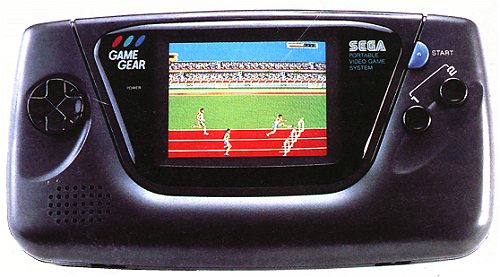
\includegraphics[scale=0.4]{../images/gamegear.png}
\caption{Sega Game Gear \protect\cite{gg}}
\label{fig:gg}
\end{figure}

The image below shows a picture of internal PCB of the Game Gear and it's major
components

\begin{table}[H]
    \centering
    \begin{tabular}{|c|l|c|l|}
        \hline
        1 & Zilog Z80 CPU           & 4 & 16K VRAM      \\ \hline
        2 & Video Display Processor & 5 & Sega BIOS ROM \\ \hline
        3 & 8K RAM                  & 6 & Controller IO \\
        \hline
    \end{tabular}
\end{table}

\newpage
\subsubsection{Functional Diagrams}
At a high level the Game Gear can be viewed simply as a system which takes
input from a game controller and produces video and audio as an output. This
description is shown in Figure~\ref{fig:external}.

\begin{figure}[H]
\centering
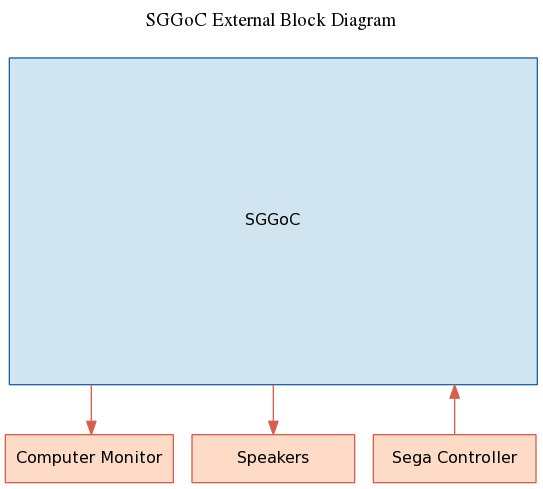
\includegraphics[scale=0.4]{../block_diagrams/block_diagram_external.png}
\caption{Black Box Diagram}
\label{fig:external}
\end{figure}

Internally the functionality can be easily modularized based on the actual
physical components found in the original Game Gear. Additional components will
be needed such as an IO controller and a memory management unit (MMU) to
account for the lack of tri-state buses in our design (explained later).
Figure~\ref{fig:internal} shows the interactions between the major functional
components in Sega Game Gear. The colored components are those which we
implemented in our project.

\begin{figure}[H]
\centering
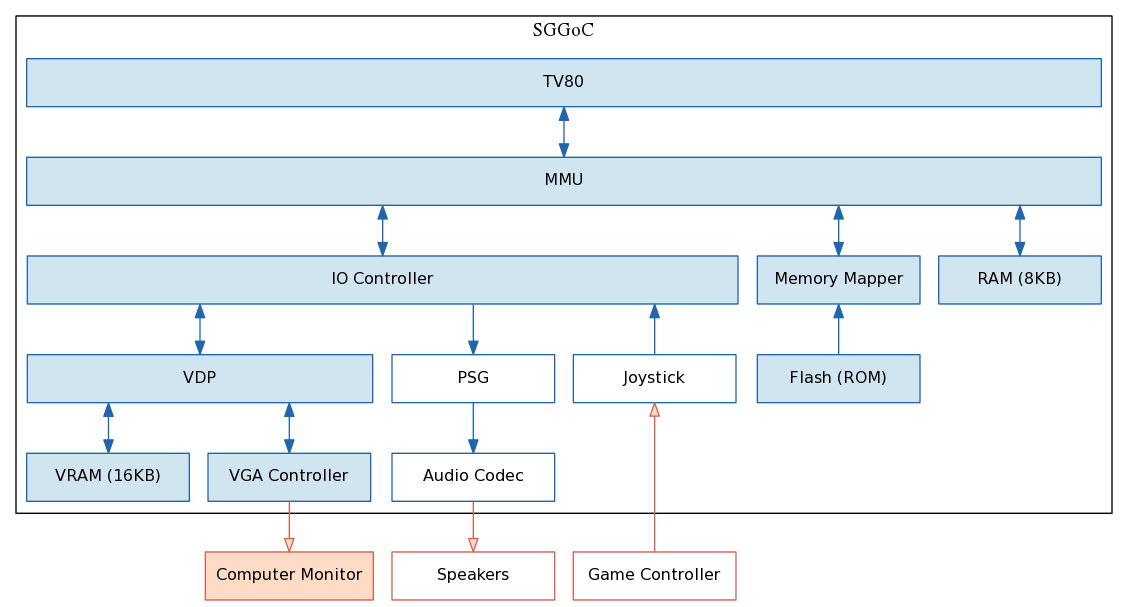
\includegraphics[scale=0.4]{../block_diagrams/block_diagram_internal_implemented.png}
\caption{Internal Functional Diagram}
\label{fig:internal}
\end{figure}

\newpage
\subsection{Cartridges and Memory Mapping}
The Z80 CPU only has 64KB of address space and 48KB of it is dedicated to the
game cartridge. A "mapper" is used to allow the use of larger ROMs (as well as
on-catridge RAM). Figure~\ref{fig:gg_cart} shows a standard GG cartridge and
Figure~\ref{fig:gg_cart_pcb} shows the internal PCB. The top chip is the Memory
Mapper and the bottom chip is the actual game ROM.

\begin{figure}[H]
    \centering
    \begin{minipage}[b]{0.3\linewidth}
        \centering
        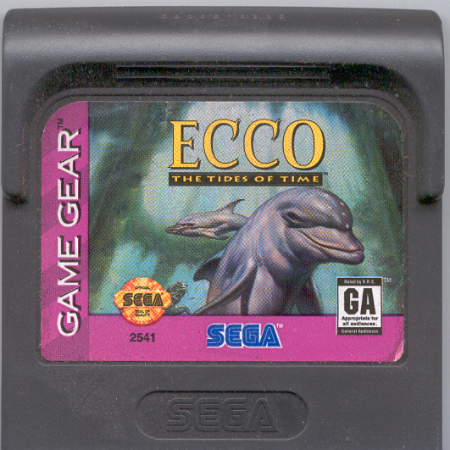
\includegraphics[height=2in]{../images/gg_cart.png}
        \caption{GG Cartridge \protect\cite{gg_cart}}
        \label{fig:gg_cart}
    \end{minipage}
    \hspace{1.5cm}
    \begin{minipage}[b]{0.3\linewidth}
        \centering
        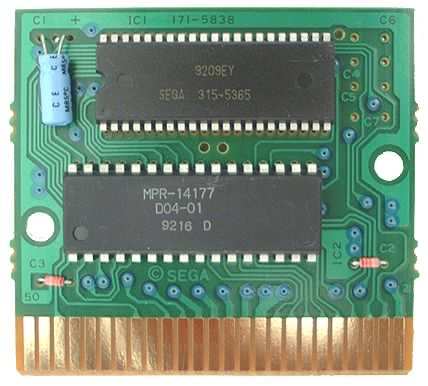
\includegraphics[height=2in]{../images/gg_cart_pcb.png}
        \caption{Cartridge PCB \protect\cite{gg_cart_pcb}}
        \label{fig:gg_cart_pcb}
    \end{minipage}
\end{figure}

\subsubsection{Sega Mapper}
There are several different mappers in existence but we only focused on
implementing the "Sega Mapper" as it is the most popular.  The Sega mapper
defines 3 16KB slots in the Z80 memory map. Any 16KB bank of ROM can be mapped
into any of these 3 slots. The mapping is controlled by memory addresses
\texttt{0xFFFC-0xFFFF}.

\begin{table}[H]
    \centering
    \begin{tabular}{ccc}
        \toprule
        \textbf{Memory Address} & \textbf{Slot} & \textbf{Maps to Z80 Address} \\
        \midrule
        \texttt{0xFFFC} & Control Bits & - \\
        \texttt{0xFFFD} & 0            & \texttt{0x0000-0x3FFF} \\
        \texttt{0xFFFE} & 1            & \texttt{0x4000-0x7FFF} \\
        \texttt{0xFFFF} & 2            & \texttt{0x8000-0xBFFF} \\
        \bottomrule
    \end{tabular}
    \caption{Mapper control registers \protect\cite{mapper}}
\end{table}

The ROM is viewed as an array of 16KB banks. The value written into the control
register determines which bank is selected for that slot.
Figure~\ref{fig:mapping_diagram} shows an example of how the address space gets
mapped to different ROM banks.

\begin{figure}[H]
\centering
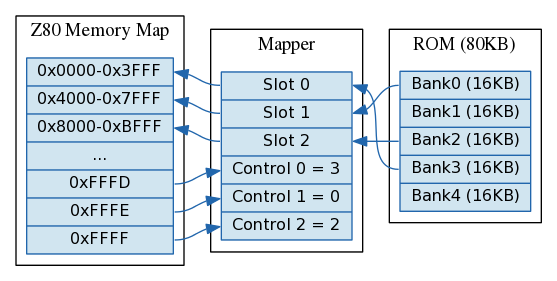
\includegraphics[height=1.5in]{../images/mapper.png}
\caption{Mapping Diagram}
\label{fig:mapping_diagram}
\end{figure}

\subsubsection{Cartridge Alternatives}
Since we are targeting a standard FPGA development board we cannot easily use
the actual game cartridge without some kind of hardware adaptor.  Additionally,
using the actual game cartridge would go against what we are trying to
accomplish with this project which is to eliminate the need for any of the
original hardware. Lucky, virtually every Game Gear cartridge has been dumped
and are available online.  Unfortunately, the ROMs range in size all the way up
to 4MB and being that most affordable FPGAs do not have that much block RAM it
would be impossible for us to pack the ROM with the bitstream. A more ideal
solution would be to use a SD card which can be loaded with numerous ROM files
and then write a bootloader to select which one to play.  The complexity of
that strategy, however, was not worth the initial effort. A simpler solution
which allowed us to quickly start on the rest of the project is to load a
single ROM file onto the Flash chip that comes with our DE-1 development board.

\subsubsection{ROM Flasher}
The technical requirements of interfacing with the flash chip on our board are
outside the scope of our project and as such we utilized a core provided by
Altera \cite{flash_core} to simplify the process.  Figure~\ref{fig:flash_core}
shows the black box diagram of the flash core provided by Altera.

\begin{figure}[H]
\centering
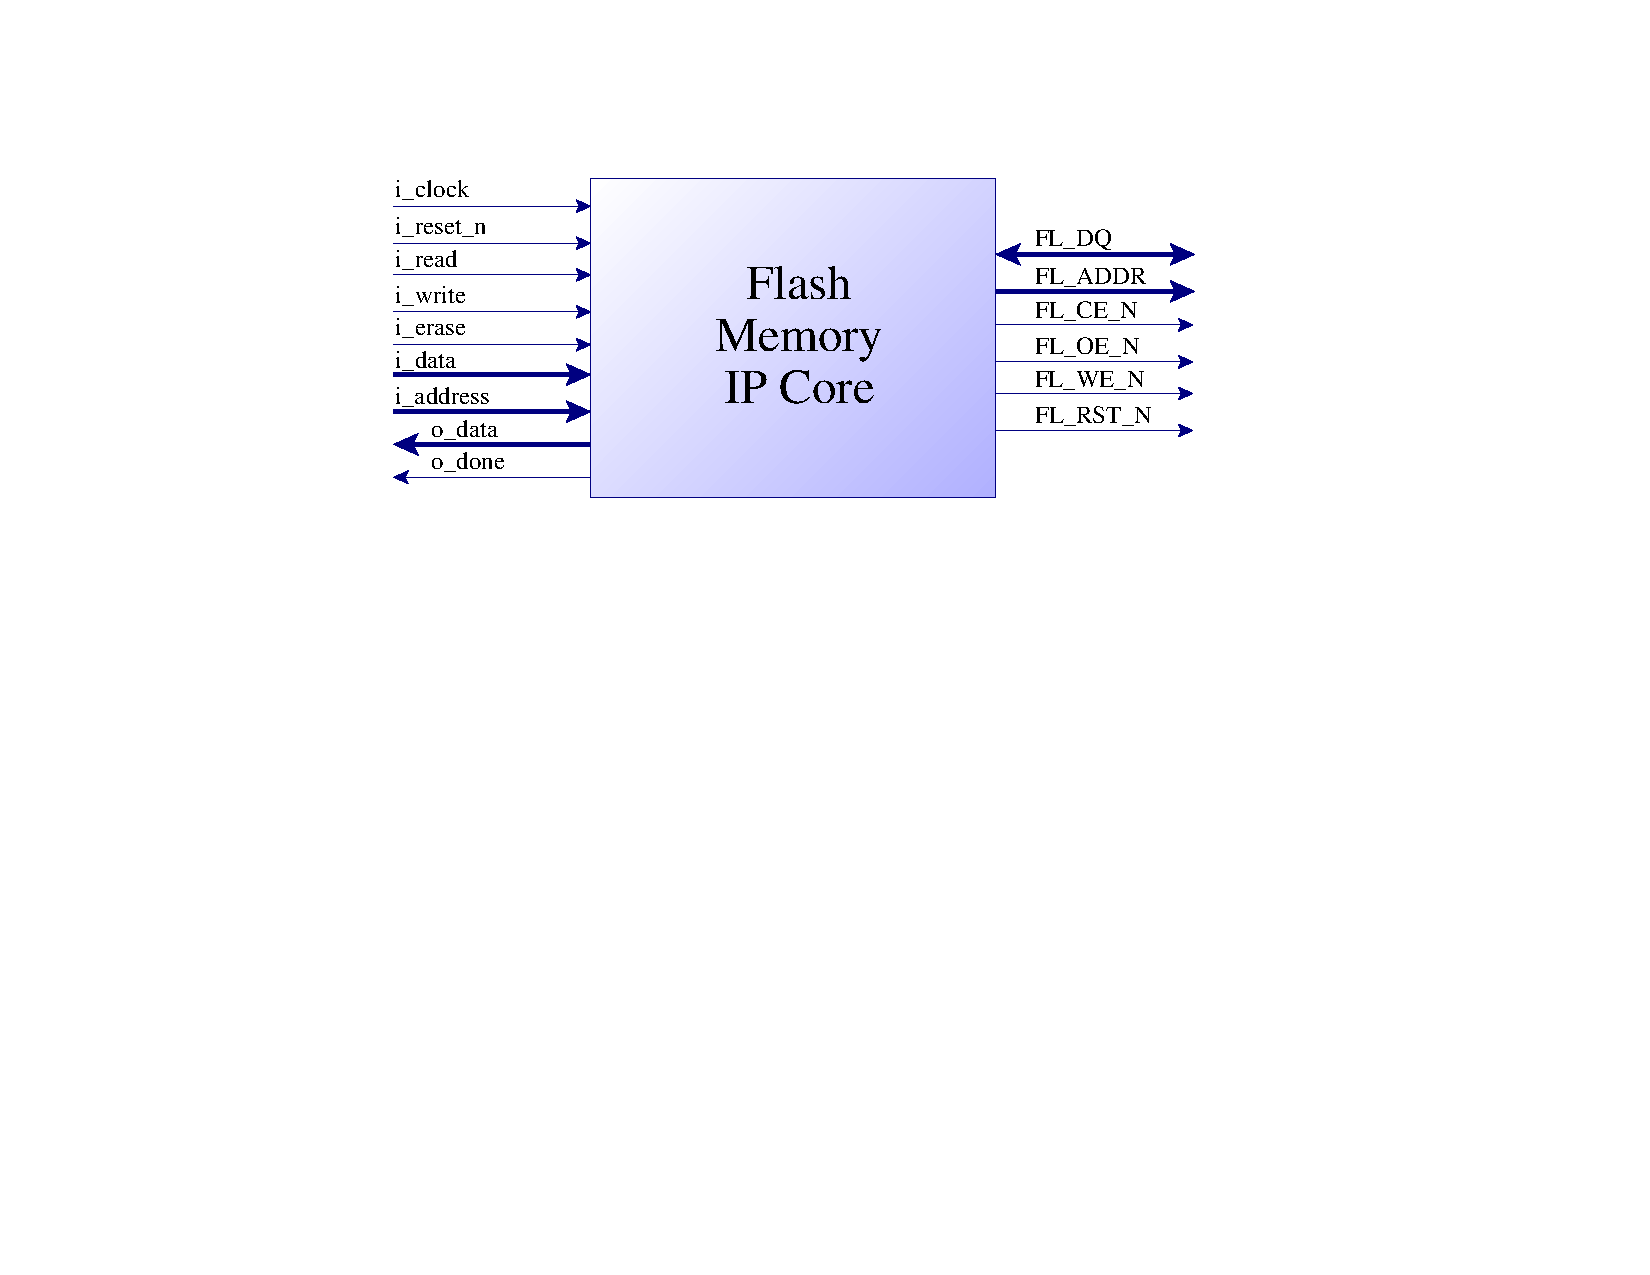
\includegraphics[scale=0.5]{../images/flash_core.pdf}
\caption{Altera Flash Core}
\label{fig:flash_core}
\end{figure}

A ``MemSend" project, completely separate from the GG project, is used to
initially load a single ROM file into the flash chip.  On the computer a Python
program reads a ROM file byte by byte and sends it to the FPGA over the serial
port. The FPGA sends back the byte it just received as an acknowledgement.
Another Python program is used to read back and verify that the flash contents
match the ROM file. Figures~\ref{fig:rom_write} and~\ref{fig:rom_read}
illustrate the process of writing and reading a ROM to and from the flash
memory.

\begin{figure}[H]
    \centering
    \begin{minipage}[b]{0.45\linewidth}
        \centering
        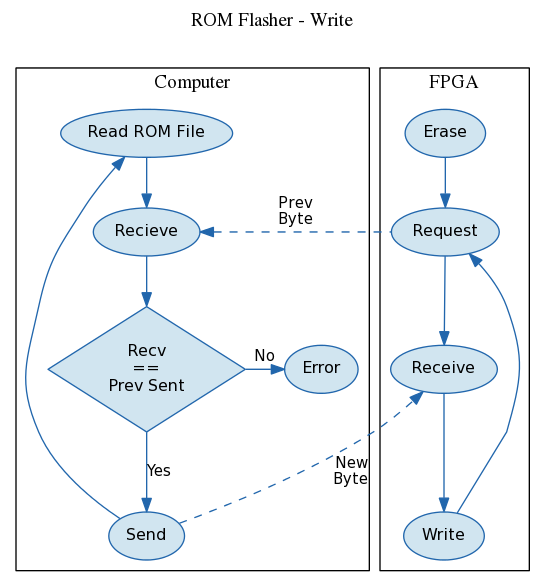
\includegraphics[width=\textwidth, height=3in]{../../fpga/rom_flasher/doc/block_diagram_write.png}
        \caption{MemSend - Write}
        \label{fig:rom_write}
    \end{minipage}
    \hfill
    \begin{minipage}[b]{0.45\linewidth}
        \centering
        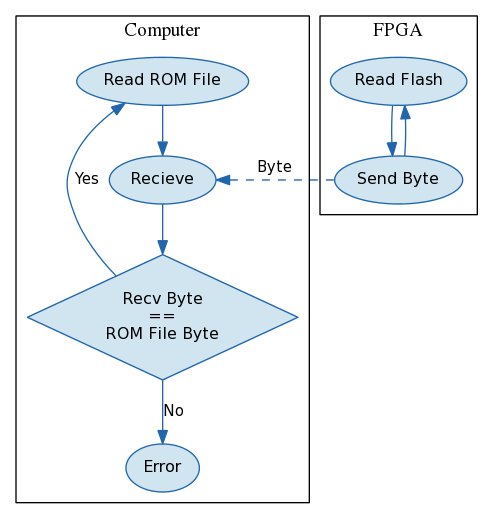
\includegraphics[width=\textwidth, height=3in]{../../fpga/rom_flasher/doc/block_diagram_read.png}
        \caption{MemSend - Read}
        \label{fig:rom_read}
    \end{minipage}
\end{figure}

\subsection{Zilog Z80}
The Game Gear uses the classic Zilog Z80 CPU running at 3.58MHz as it's main
processor.  The re-implementation of the Z80 is completely outside the scope of
this project and as such we utilized the popular TV80 \cite{tv80} CPU which is
a proven, open source, implementation of the Z80 written in Verilog.  The
interface of the TV80 exactly matches that of the original Z80, shown in
Figure~\ref{fig:z80}, with the only exception being the data bus. The original
Z80, as well as the whole Game Gear memory system, relies on tri-state buses
where as the TV80 has a separate bus for data in and data out.

\begin{figure}[H]
\centering
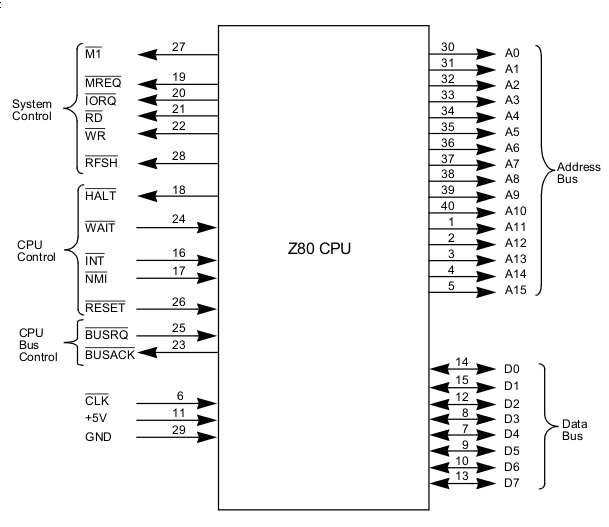
\includegraphics[scale=0.4]{../images/z80.png}
\caption{Zilog Z80}
\label{fig:z80}
\end{figure}

\subsection{Memory Management Unit (MMU)}
Since our design does not use tri-state buses we cannot simply connect the data
lines from each component together. Instead, we need to have some kind of
memory manager that can multiplex the data lines to whichever device the
address is pointing to according the system memory map. The full memory map for
the Game Gear is shown below

\begin{table}[H]
    \centering
    \begin{tabular}{ll}
        \toprule
        \textbf{Address} & \textbf{Device} \\
        \midrule
        \texttt{0x0000-0x03FF} & ROM (unpaged)                    \\
        \texttt{0x0400-0x3FFF} & ROM mapper slot 0                \\
        \texttt{0x4000-0x7FFF} & ROM mapper slot 1                \\
        \texttt{0x8000-0xBFFF} & ROM mapper slot 2 - OR - SaveRAM \\
        \texttt{0xC000-0xDFFF} & System RAM                       \\
        \texttt{0xE000-0xFFFF} & System RAM (mirror)              \\
        \texttt{0xFFFC}       & SaveRAM mapper control           \\
        \texttt{0xFFFD}       & Mapper slot 0 control            \\
        \texttt{0xFFFE}       & Mapper slot 1 control            \\
        \texttt{0xFFFF}       & Mapper slot 2 control            \\
        \bottomrule
    \end{tabular}
    \fontfamily{}\selectfont
    \caption{Z80 Memory Map \protect\cite{mem_map_table}}
\end{table}

Since the cartridge mapper handles the slot mapping itself we are really
only multiplexing between the cartridge, the system RAM, and the IO controller
which share the memory bus.  The system RAM happens to start at a nice edge
being that \texttt{0xC000 = 0b1100000000000000}. To see if we are accessing RAM
we only need to check to see if bits 15 and 16 are high. If so, we can simply
use the 13 LSBs of the Z80 address as the index into the RAM.  This method also
accounts for the RAM mirror since the 13 LSBs repeat starting at 0xE000.

\subsection{IO Controller}

The IO Controller is responsible for determining which IO port
the Z80 is currently reading or writing from during an IO operation.
The port that is currently selected is decoded to one of 8 possible
ports using address bits 7, 6, and 0. The following table describes
which port corresponds to which IO device.

\begin{table}[H]
    \centering
    \begin{tabular}{cl}
        \toprule
        \textbf{IO Port} & \textbf{Device} \\
        \midrule
        \texttt{0} & Memory Control \\
        \texttt{1} & IO Port Control\\
        \texttt{2} & VDP V Counter \\
        \texttt{3} & VDP H Counter \\
        \texttt{4} & VDP Data \\
        \texttt{5} & VDP Control \\
        \texttt{6} & Input A/B \\
        \texttt{7} & Input B/Misc \\
        \bottomrule
    \end{tabular}
    \caption{IO Port Mapping}
\end{table}

The IO controller is also responsible for generating the VDP control and
data read write signals.

\subsection{Video Display Processor (VDP)}

The Video Display Processor is a graphics chip which is derived from a Texas
Instruments TMS9918. The VDP contains 10 control registers and interfaces with
16KB of VRAM which it reads from to continuously draw the background and sprite
tiles to the screen. The Z80 can only access the VRAM through the \texttt{Data}
and \texttt{Control} IO ports. Additionally, the VDP provides a vertical and
horizontal pixel count which is accessed by the Z80 via the \texttt{V Counter}
and \texttt{H Counter} IO ports.  Finally, the VDP directly drives the
interrupt line of the Z80 and asserts an interrupt when certain video events
have occurred.

\subsubsection{Control Port}

The VDP is programmed by sending a two-byte sequence to the control port. The
control port is used to define an offset into VRAM or CRAM for subsequent data
port I/O, and also to write to the internal VDP registers.

There is a flag which is set after the first byte is sent and cleared when the
second byte is written. This insures the VDP knows which byte of the control
port is being received. The flag is also cleared when the control port is read
or when the data port is read or written.

The address register is 14 bits in length and defines the address into VRAM
for reads and writes and the address into CRAM for writes. The code register
is 2 bits in length and selects four different operations.

Writes to the control port have the following format:

\begin{figure}[H]
    \centering
    \begin{bytefield}[bitwidth=2em, endianness=big]{8}
        \begin{rightwordgroup}{First Byte Written}
            \bitbox{1}{\tiny A07} & \bitbox{1}{\tiny A06} & \bitbox{1}{\tiny A05} & \bitbox{1}{\tiny A04} &
            \bitbox{1}{\tiny A03} & \bitbox{1}{\tiny A02} & \bitbox{1}{\tiny A01} & \bitbox{1}{\tiny A00}
        \end{rightwordgroup} \\
        \bitheader{0-7} \\
        \begin{rightwordgroup}{Second Byte Written}
            \bitbox{1}{\tiny CD1} & \bitbox{1}{\tiny CD0} & \bitbox{1}{\tiny A13} & \bitbox{1}{\tiny A12} &
            \bitbox{1}{\tiny A11} & \bitbox{1}{\tiny A10} & \bitbox{1}{\tiny A09} & \bitbox{1}{\tiny A08}
        \end{rightwordgroup} \\
        \bitheader{0-7}
    \end{bytefield}
\end{figure}

Where,

\begin{table}[H]
    \centering
    \begin{tabular}{ll}
        \toprule
        \textbf{Bits} & \textbf{Definition} \\
        \midrule
        CDx & Code register     \\
        Axx & Address register  \\
        \bottomrule
    \end{tabular}
\end{table}

When the first byte is written it is stored in a temporary hold register.  Once
the second byte is written the code is checked to see if it is setting the VRAM
address or doing a register write. If it is setting the VRAM then the temporary
hold register is used to update the lower 8 bytes of the VRAM address and the
lower 6 bites of the second byte are used to update the upper bits of the VRAM
address.

The table below summarizes the different actions performed for each code.

\begin{table}[H]
    \centering
    \begin{tabular}{clp{3.5in}}
        \toprule
        \textbf{Code} & \textbf{Action} & \textbf{Description}\\
        \midrule
        0 & VRAM Read       & A byte of VRAM is read from the location defined by
                              the address register and is stored in the read buffer.
                              The address register is incremented by one. Writes to
                              the data port go to VRAM.                                     \\
        1 & VRAM Write      & Writes to the data port go to VRAM                            \\
        2 & Register Write  & This value signifies a VDP register write, explained below.
                              Writes to the data port go to VRAM.                           \\
        3 & CRAM Write      & Writes to the data port go to CRAM.                           \\
        \bottomrule
    \end{tabular}
\end{table}

When accessing CRAM, the upper bits of the address register are ignored as the
CRAM is only 64 bytes. The address register will wrap when it exceeds \texttt{0x3FFF}.

If the code specified by the second byte indicates a register write the two
bytes have a different format as shown below.

\begin{figure}[H]
    \centering
    \begin{bytefield}[bitwidth=2em, endianness=big]{8}
        \begin{rightwordgroup}{First Byte Written}
            \bitbox{1}{\tiny D07} & \bitbox{1}{\tiny D06} & \bitbox{1}{\tiny D05} & \bitbox{1}{\tiny D04} &
            \bitbox{1}{\tiny D03} & \bitbox{1}{\tiny D02} & \bitbox{1}{\tiny D01} & \bitbox{1}{\tiny D00}
        \end{rightwordgroup}\\
        \bitheader{0-7} \\
        \begin{rightwordgroup}{Second Byte Written}
            \bitbox{1}{\tiny 1}   & \bitbox{1}{\tiny 0}   & \bitbox{1}{\tiny X}   & \bitbox{1}{\tiny X} &
            \bitbox{1}{\tiny R03} & \bitbox{1}{\tiny R02} & \bitbox{1}{\tiny R01} & \bitbox{1}{\tiny R00}
        \end{rightwordgroup} \\
        \bitheader{0-7}
    \end{bytefield}
\end{figure}

Where,

\begin{table}[H]
    \centering
    \begin{tabular}{ll}
        \toprule
        \textbf{Bits} & \textbf{Definition} \\
        \midrule
        Rxx & Register number   \\
        Dxx & Register data     \\
        x   & Ignored           \\
        \bottomrule
    \end{tabular}
\end{table}

The VDP selects a register using bits 3-0 of the second byte and writes the
data from the first byte into that register. Since there is only 10 registers
values 11 through 15 have no effect when written to.

\subsubsection{Data Port}

Depending on the code register, data written to the data port is sent to either
VRAM or CRAM. After each write, the address register is incremented by one, and
will wrap past \texttt{3FFF}.

Reads from VRAM or CRAM are buffered. Every time the data port is read
(regardless of the code register) the contents of a buffer are returned. The
VDP will then read a byte from VRAM at the current address, and increment the
address register.  In this way data for the next data port read is ready with
no delay while the VDP reads VRAM.

\subsubsection{Status Flags}

Reading the control port returns a byte containing status flags:

\begin{figure}[H]
    \centering
    \begin{bytefield}[bitwidth=2em, endianness=big]{8}
        \bitbox{1}{\tiny INT} & \bitbox{1}{\tiny OVR} & \bitbox{1}{\tiny COL} & \bitbox{1}{\tiny ---} &
        \bitbox{1}{\tiny ---} & \bitbox{1}{\tiny ---} & \bitbox{1}{\tiny ---} & \bitbox{1}{\tiny ---} \\
        \bitheader{0-7}
    \end{bytefield}
    \caption{Status Register}
\end{figure}

The \textbf{INT} bit indicates a frame interrupt is pending and is set on the
first line after the end of the active display period. It is cleared when the
control port is read. (See the interrupts section for more details). The
\textbf{OVR} and \textbf{COL} bits are used for sprites and are not implemented
in our project. The remaining bits are not set by the VDP.

\subsubsection{Color RAM (CRAM)}

The Game Gear uses a 64 byte palette where each entry is composed of two bytes as shown below.

\begin{figure}[H]
    \centering
    \begin{bytefield}[bitwidth=2em, endianness=big]{8}
        \begin{rightwordgroup}{High byte}
        \bitbox{1}{\tiny --} & \bitbox{1}{\tiny --} & \bitbox{1}{\tiny --} & \bitbox{1}{\tiny --} &
        \bitbox{1}{\tiny B3} & \bitbox{1}{\tiny B2} & \bitbox{1}{\tiny B1} & \bitbox{1}{\tiny B0}
        \end{rightwordgroup}\\
        \bitheader{0-7}
        \\
        \begin{rightwordgroup}{Low byte}
        \bitbox{1}{\tiny G3} & \bitbox{1}{\tiny G2} & \bitbox{1}{\tiny G1} & \bitbox{1}{\tiny G0} &
        \bitbox{1}{\tiny R3} & \bitbox{1}{\tiny R2} & \bitbox{1}{\tiny R1} & \bitbox{1}{\tiny R0}
        \end{rightwordgroup}\\
        \bitheader{0-7}
    \end{bytefield}
    \caption{Palette Entry}
\end{figure}

When writing to CRAM the address register wraps at \texttt{0x0040}. Writing to
an even CRAM address causes the data written to be stored in a latch, and
writing to an odd CRAM address makes the VDP write the contents of the latch as
well as the new data from the CPU to the current CRAM entry.

Therefore, writing single bytes to even CRAM addresses will not modify CRAM.
You could write multiple times to even addresses. This allows the same latched
color data to be written to multiple palette entries.

\subsubsection{Display Modes}

The TMS9918 has three bits which select different display modes called M1, M2,
and M3. Note that in the TMS9918 manual, there are only four modes documented:

\begin{table}[H]
    \centering
    \begin{tabular}{l c c l}
        Mode & 0 & - & Graphics I   \\
        Mode & 1 & - & Text         \\
        Mode & 2 & - & Graphics II  \\
        Mode & 3 & - & Multicolor   \\
    \end{tabular}
\end{table}

%\subsection{Tiles}
%\subsection{Layers}
\subsubsection{Counters}

The VDP is responsible for two counters:

\begin{enumerate}
    \item \textbf{Horizontal Counter,}
    \item \textbf{Vertical Counter.}
\end{enumerate}

The horizontal counter is incremented on the rising edge of the VGA clock. Once
each scanline is complete, the vertical counter is then incremented by one, and
this continues until a full frame is generated.

The horizontal and vertical counters can be read by the Z80. Also, the vertical
counter can be read at any time. Our design consisted of using a NTSC display of
256x192. Description of the line values can be shown below:

\begin{table}[H]
    \centering
    \begin{tabular}{l|l}
        Lines   & Description       \\ \hline \hline
        192     & Active Display    \\
        24      & Bottom Border     \\
        3       & Bottom Blanking   \\
        3       & Vertical Blanking \\
        13      & Top Blanking      \\
        27      & Top Border        \\
    \end{tabular}
\end{table}

Vertical counter values:

\vspace{-0.1cm}
\begin{itemize}
    \item 00  - 218,
    \item 213 - 255.
\end{itemize}

\subsubsection{Interrupts}

The VDP generates two interrupts:

\vspace{-0.1cm}
\begin{enumerate}
    \item \textbf{Frame interrupt:} occurs when vertical blanking period has started,
    \item \textbf{Line interrupt:} occurs when the line interrupt counter has expired.
\end{enumerate}

\textbf{\underline{Frame Interrupts }}

There are several different height displays, and depending on each one, the VDP will
generate a frame interrupt on the following lines:

\begin{table}[H]
    \centering
    \begin{tabular}{c|c}
        Height  & Line \\ \hline \hline
        192     & 0xC1 \\
        224     & 0xE1 \\
        240     & 0xF1 \\
    \end{tabular}
\end{table}

Depending on the height, for example, we used a height of 192 in our design, an
interrupt at line 193 (0xC1) will be raised and the VDP will set bit 7 of the status
flags. This bit will remain set until the control port is read.

The fifth bit of the first register acts like a toggle switch for the VDP's interrupt
request (IRQ) line. Therefore if the 5th bit of register 1 is set and the 7th bit of
the status flag is set, the VDP will assert the IRQ line, and if that bit is cleared,
then the VDP will de-assert the IRQ line.

\textbf{\underline{Line Interrupts }}

The contents of the 10th register is loaded into a counter on every line outside of
the active display period which excludes the line after the last line of the active
display period. The counter is then decremented on every line within the active display
period including the line after the last line of the active display period.

For example, with a 192-line display on a NTSC machine that has 262 scanlines per
frame (used in our design):

For lines 0 - 261:

\vspace{-0.1cm}
\begin{enumerate}
    \item The counter is decremented on lines 0 - 192,
    \item Then the counter is reloaded on lines 193 - 261.
\end{enumerate}

If the counter underflows from 0 to 255, then it is reloaded with the previous contents
stored in register 10. Writing to the tenth register will not immediately affect/change
the contents of the counter; this only occurs when the VDP is outside of the active
display or when (counter is reloaded) or when the counter underflows.

The VDP sets an internal flag when the counter underflows. This flag remains set until
the control port is read.

The fourth bit of register 0 acts like a toggle switch for the VDP's IRQ line. If the
internal flag is set and the fourth bit of register 0 is set, then the VDP will assert
the IRQ line, and will de-assert the IRQ line if the bit is cleared.

%\subsection{Display Timing}
\subsection{VGA Controller}

\newpage
\section{Test Plan}

\subsection{VDP Background Generation}

In order to test the operation of the VDP background generator a separate test
project was used which only consists of the background generator, VRAM, VGA timing
generator, and a UART interface.

Games are run using the open-source Osmose Sega Emulator \cite{osmose}. When
the game reaches a screen that we want to test on the FPGA we dump the VRAM and
CRAM using Osmoses built in debugger. We then use programs, written in C, that
read the VRAM dump and generate images of the color palette, all 512 background
tiles, and the final screen rendering.  These programs serve a dual purpose
allowing us to both confirm our understanding of how the background image is
generated and also that our VRAM dump is valid. The images below show example
output from these three programs.
\vfill
\begin{figure}[H]
    \centering
    \begin{minipage}[H]{0.45\linewidth}
        \centering
        
\includegraphics[width=\textwidth]{../images/palette.png}
        \caption{Color Palette}
        \label{fig:palette}
    \end{minipage}
    \hfill
    \begin{minipage}[H]{0.45\linewidth}
        \centering
        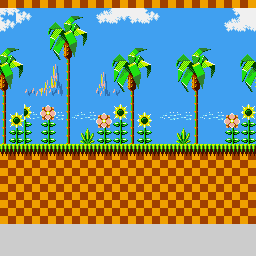
\includegraphics[width=\textwidth]{../images/screen.png}
        \caption{Complete Screen Render}
        \label{fig:screen}
    \end{minipage}
\end{figure}
\vfill
\begin{figure}[H]
    \centering
    \begin{minipage}[H]{0.8\linewidth}
        \centering
        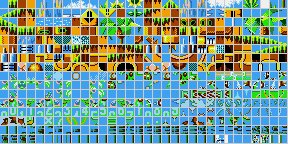
\includegraphics[width=\textwidth]{../images/tiles.png}
        \caption{All 512 Tiles}
        \label{fig:tiles}
    \end{minipage}
\end{figure}
\vfill
\newpage

After the VRAM dumps have been obtained they are loaded into the VRAM on the
FPGA via the same `MemSend' program introduced in the ROM section. The image
displayed on the monitor is then verified to ensure it matches both the
emulator and the output renderings of our C programs.

The testing strategy is executed as follows:
\begin{enumerate}
    \item Obtain VRAM dump from the Osmose emulator
        \begin{enumerate}
            \item Launch Osmose and open ROM file
                \begin{verbatim}$ ./Osmose-0-9-96-QT sonic.gg\end{verbatim}
            \item Set a scanline breakpoint in the debug console
                \begin{verbatim}Cmd: slbp 20\end{verbatim}
            \item Continue execution by entering `c' until the desired frame is reached.
            \item Dump the VRAM and CRAM
                \begin{verbatim}Cmd: davram 0\end{verbatim}
            \item Dump files are located at \texttt{/tmp/osmose.(vram,cram)}
        \end{enumerate}
    \item Verify dump integrity using C rendering programs
        \begin{enumerate}
            \item Run \texttt{screen}, located in \texttt{./tools/vdp\_render/}, on the dump files
            \item Ensure \texttt{screen.png} is generated
            \item Inspect \texttt{screen.png} pixel by pixel to ensure it matches the frame displayed in Osmose
            \item If image does not match another dump must be performed
            \item If image still does not match then debugging needs to be performed on the \texttt{screen} rendering program
        \end{enumerate}
    \item Transfer dump to FPGA VRAM via the `MemSend' tool
        \begin{enumerate}
            \item Flash the FPGA with the Video Display Processor test project located in \texttt{./fpga/vdp\_test/}
            \item Send a ROM file to the FPGA via the \texttt{send.py} program located in \texttt{./tools/mem\_send/}
            \item Ensure the \texttt{send.py} program completes without errors
        \end{enumerate}
    \item Verify that resulting image on screen
        \begin{enumerate}
            \item Inspect resulting image on monitor pixel by pixel and verify it matches both the original Osmose frame as well as the output from the C rendering programs
            \item If the image doe not match attempt to resend the rom
            \item If the image still does not match then debugging needs to be performed on the image rendering core.
        \end{enumerate}
\end{enumerate}

\subsection{Custom Test ROMs}

In order to test the operation of the z80, and basic functionality of the VDP,
custom ROMs were developed. Using the Small Device C Compiler (SDCC)
\cite{SDCC} we are able to write programs that exercises various functionality
of the system.

We found SDCC extremely easy to setup and get working. The only thing
we needed to modify was the initial stack pointer value in the C
Runtime file (crt0.s). The default stack pointer location is set to
\texttt{0xFFFF} but the top most RAM address on the Game Gear is
\texttt{0xDFFF}. Setting up IO is as easy as specifying a special
function register at a given IO port. An example showing how to write
data to the VDP data port (0xBE) is shown below.

\begin{lstlisting}[caption=VDP Data Write]
    __sfr __at (0xBE) vdp_data;
    int main() {
        vdp_data = 0x38;    // write 0x38 to VDP data port
        while (1) {}
        return 0;
    }
\end{lstlisting}

We ended up building a small GG library with the following functions:

\begin{lstlisting}[caption=Game Gear Library Functions]
    void vdp_write_control(uint8_t value);
    void vdp_write_data(uint8_t value);
    void vdp_set_register(uint8_t reg, uint8_t value);
    void vdp_set_vram_addr(uint16_t addr);
    void vdp_set_palette(uint8_t id, uint16_t color);
    void set_pattern_fill(uint16_t id, uint8_t color);
    void set_tile_to_pattern(uint8_t x, uint8_t y, uint16_t pattern);
    void delay(uint16_t x);
    void set_debug(uint8_t x);
\end{lstlisting}

With this library in place it is easy to to perform operations such as setting
up the color palette:

\begin{lstlisting}[caption=Color Palette Test ROM]
    #include <gg.h>
    int main() {
        // set register 1 bit 6 to enable display
        vdp_set_register(1, (1<<6));
        // set first color palette entry to gray
        vdp_set_palette(0, 0x0CCC);
        while (1) {}
        return 0;
    }
\end{lstlisting}

A few different test ROMs were developed to test drawing tiles and scrolling.
The ROMs were first run on an emulator to verify their functionality before
being loaded into flash on the FPGA board. The output of the `tiles' test ROM
is shown below:

\begin{figure}[H]
    \centering
    \begin{minipage}[H]{0.45\linewidth}
        \centering
        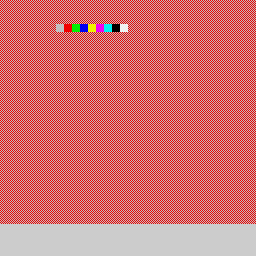
\includegraphics[width=\textwidth]{../images/tiles_screen.png}
        \caption{Tiles Screen}
        \label{fig:tiles_screen}
    \end{minipage}
    \hfill
    \begin{minipage}[H]{0.45\linewidth}
        \centering
        
\includegraphics[width=\textwidth]{../images/tiles_palette.png}
        \caption{Tiles Palette}
        \label{fig:tile_palette}
    \end{minipage}
\end{figure}

The general testing strategy for the test ROMs is executed as follows:

\begin{enumerate}
    \item Identify a specific functionality that you wish to test (scrolling the background left by 5 pixels for example)
    \item Write a test program that achieves the desired functionality in the simplest way possible.
    \item Run the test program in the Osmose emulator and ensure the test program achieves the desired functionality.
    \item Flash the test ROM onto the FPGA development board using the `MemSend' tool.
    \item Verify that the desired functionality is also achieved on the FPGA.
\end{enumerate}

\subsection{Simulation vs Emulator}

In order to prove that our system is functionality equivalent to a known `good'
system we utilized simulations to generate dumps of all major events happening
in the system. The events that we are primarily concerned with are memory and
IO accesses. In order to generate logs of all the events we inserted prints
into our simulation when the desired events occurred. We then inserted the
exact same print into the emulator. By running the same game in both the
simulation and the emulator we can compare the difference between the print
logs and identify differences in functionality.

The testing strategy for this testing method is executed as follows:

\begin{enumerate}
    \item Insert print statements on all memory and IO accesses in the emulator
    \item Insert the exact same print statements on all memory and IO accesses in the simulation
    \item Run the emulator and simulation on the same ROM
    \item Diff the resulting logs
    \item Verify that the memory and IO accesses match between the emulator and simulation
\end{enumerate}

An example of a successful test result is shown below in
Figure~\ref{fig:diff_good}. Notice how both the simulation and emulator prints
indicate matching functionality.

\begin{figure}[H]
\centering
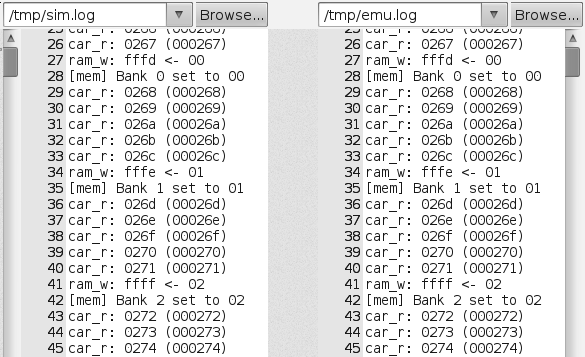
\includegraphics[scale=0.4]{../images/diff_good.png}
\caption{Successful Test Result}
\label{fig:diff_good}
\end{figure}

On the contrary Figure~\ref{fig:diff_bad} shows an example of a bad test
result. Notice how there are discrepancies between the simulation (shown on the left) and the
emulator (shown on the right).

\begin{figure}[H]
\centering
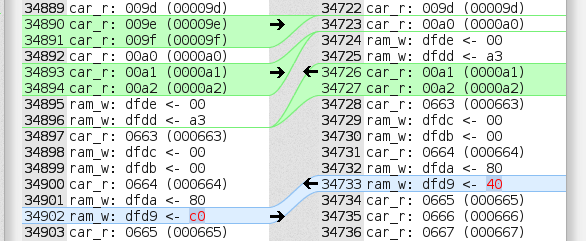
\includegraphics[scale=0.4]{../images/diff_bad.png}
\caption{Successful Test Result}
\label{fig:diff_bad}
\end{figure}
\section{Project Limitations}

Our project currently has a few limitations the most notable of which is
missing core functionality.  The Video Display Processor does not currently
implement sprite tiles which makes most games unplayable due to the fact
that the actual game characters, items, and enemies are often drawn as sprites.
We also did not have time to fully implement controller support or audio
support. These features are incomplete purely due to lack of time not technical
problems with them. With time all components found in the original Game Gear
will be implemented.

Another issue that currently exists in our project is video corruption. Tiles are
sometimes flipped or the wrong tile is drawn. This corruption differs between game
but seems to be static per game in that the game is corrupted the same way each
time. Interestingly, some games have significantly more corruption than others.
Our current guess is that there is a timing issue in the video display
processor. We also believe that there might be a logic issue in the way the
video display processor generates interrupts. In order to combat this issue we
plan to try and create a custom test ROM which can consistently replicate the
issue.  We hope that we will then be able to narrow down the root cause by
using similar debugging techniques discussed above such as comparing simulation
results to an emulator.

An additional limitation, while not critical to the overall functionality of
our project, is the fact that loading a new game ROM onto the board is
cumbersome and time consuming. The method that is currently implemented was
originally chosen because of it's relative simplicity in implementation and
allowed us to quickly move on to the rest of the development.  A better
solution in the long run would be to write a simple bootloader that loads game
ROMs into RAM off an SD card. This would allow us to store multiple games on
the SD card and simply choose which one we wanted to run on startup.

\section{Social Responsibility}

\textbf{Copyright and liscensing} were two concerns for us throughout this
project.  Part of our project deals with using game ROMs that we downloaded off
the internet which raises a copyright issue. While it is illegal to create a
full duplicate of the original media it is generally understood that possessing
a ROM dump of a game you physically own is acceptable. For our project we tried
to only use game ROMs of games that we physically own. Two other components of
our project, the TV80 CPU and the Osmose emulator, are open sourced under the
GPL license. One of the main objective of the license is to ensure that
derivatives of the project are also released as open source. This was a
non-issue for us since our entire project shares the GPL license as well.

\textbf{Reasonable cost and maintainability} were two of the main driving
factors of our project. The primary idea of our project is to show that it is
beneficial to re-implement legacy systems in an FPGA. We believe that
re-implementation can be done at a reasonable cost being that the physical
hardware needed for an FPGA solution is cheaper than it has ever been before
and the only other cost overhead is development man-hours. The cost trade off
between re-implementation and monetary loss due to a legacy system failing
swings towards re-implementation being more beneficial. Re-implementation in a
FPGA also opens the door to better maintainability given that the system is no
longer dependant on physical, deprecated, components.

\section{Conclusion}

\newpage
\begin{thebibliography}{9}
    \bibitem{gg} \url{http://mo5.com/musee-machines-gamegear.html}
    \bibitem{gg_cart} \url{http://www.magisterrex.com/prodimages/EccoDolphinGameGear-h450.png}
    \bibitem{gg_cart_pcb} \url{http://www.smspower.org/Development/SMSPagingChips}
    \bibitem{mapper} \url{http://www.smspower.org/Development/Mappers}
    \bibitem{flash_core} \url{ftp://ftp.altera.com/up/pub/flash/altera_up_flash_memory.zip}
    \bibitem{tv80} \url{http://opencores.org/project,tv80}
    \bibitem{mem_map_table} \url{http://code.google.com/p/bizhawk/source/browse/trunk/BizHawk.Emulation/Consoles/Sega/SMS/MemoryMap.Sega.cs}
    \bibitem{VDP} \url{http://www.smspower.org/uploads/Development/msvdp-20021112.txt?sid=c8bdf72dd28a0a34eeedf5f7742ca62a}
    \bibitem{osmose} \url{http://bcz.asterope.fr/osmose.htm}
    \bibitem{ieeeverilog} \url{http://ieeexplore.ieee.org/stamp/stamp.jsp?arnumber=00954909}
    \bibitem{gpl} \url{http://www.gnu.org/licenses/gpl.html}
    \bibitem{SDCC} \url{http://sdcc.sourceforge.net/}
\end{thebibliography}

\end{document}
